\documentclass[a4paper,11pt]{article}
\usepackage[a4paper, margin=8em]{geometry}

% usa i pacchetti per la scrittura in italiano
\usepackage[french,italian]{babel}
\usepackage[T1]{fontenc}
\usepackage[utf8]{inputenc}
\frenchspacing 

% usa i pacchetti per la formattazione matematica
\usepackage{amsmath, amssymb, amsthm, amsfonts}

% usa altri pacchetti
\usepackage{gensymb}
\usepackage{hyperref}
\usepackage{standalone}

\usepackage{colortbl}

\usepackage{xstring}
\usepackage{karnaugh-map}

% imposta il titolo
\title{Appunti Ingegneria del Software}
\author{Luca Seggiani}
\date{2025}

% imposta lo stile
% usa helvetica
\usepackage[scaled]{helvet}
% usa palatino
\usepackage{palatino}
% usa un font monospazio guardabile
\usepackage{lmodern}

\renewcommand{\rmdefault}{ppl}
\renewcommand{\sfdefault}{phv}
\renewcommand{\ttdefault}{lmtt}

% circuiti
\usepackage{circuitikz}
\usetikzlibrary{babel}

% testo cerchiato
\newcommand*\circled[1]{\tikz[baseline=(char.base)]{
            \node[shape=circle,draw,inner sep=2pt] (char) {#1};}}

% disponi il titolo
\makeatletter
\renewcommand{\maketitle} {
	\begin{center} 
		\begin{minipage}[t]{.8\textwidth}
			\textsf{\huge\bfseries \@title} 
		\end{minipage}%
		\begin{minipage}[t]{.2\textwidth}
			\raggedleft \vspace{-1.65em}
			\textsf{\small \@author} \vfill
			\textsf{\small \@date}
		\end{minipage}
		\par
	\end{center}

	\thispagestyle{empty}
	\pagestyle{fancy}
}
\makeatother

% disponi teoremi
\usepackage{tcolorbox}
\newtcolorbox[auto counter, number within=section]{theorem}[2][]{%
	colback=blue!10, 
	colframe=blue!40!black, 
	sharp corners=northwest,
	fonttitle=\sffamily\bfseries, 
	title=Teorema~\thetcbcounter: #2, 
	#1
}

% disponi definizioni
\newtcolorbox[auto counter, number within=section]{definition}[2][]{%
	colback=red!10,
	colframe=red!40!black,
	sharp corners=northwest,
	fonttitle=\sffamily\bfseries,
	title=Definizione~\thetcbcounter: #2,
	#1
}

% disponi codice
\usepackage{listings}
\usepackage[table]{xcolor}

\definecolor{codegreen}{rgb}{0,0.6,0}
\definecolor{codegray}{rgb}{0.5,0.5,0.5}
\definecolor{codepurple}{rgb}{0.58,0,0.82}
\definecolor{backcolour}{rgb}{0.95,0.95,0.92}

\lstdefinestyle{codestyle}{
		backgroundcolor=\color{black!5}, 
		commentstyle=\color{codegreen},
		keywordstyle=\bfseries\color{magenta},
		numberstyle=\sffamily\tiny\color{black!60},
		stringstyle=\color{green!50!black},
		basicstyle=\ttfamily\footnotesize,
		breakatwhitespace=false,         
		breaklines=true,                 
		captionpos=b,                    
		keepspaces=true,                 
		numbers=left,                    
		numbersep=5pt,                  
		showspaces=false,                
		showstringspaces=false,
		showtabs=false,                  
		tabsize=2
}

\lstdefinestyle{shellstyle}{
		backgroundcolor=\color{black!5}, 
		basicstyle=\ttfamily\footnotesize\color{black}, 
		commentstyle=\color{black}, 
		keywordstyle=\color{black},
		numberstyle=\color{black!5},
		stringstyle=\color{black}, 
		showspaces=false,
		showstringspaces=false, 
		showtabs=false, 
		tabsize=2, 
		numbers=none, 
		breaklines=true
}


\lstdefinelanguage{assembler}{ 
  keywords={AAA, AAD, AAM, AAS, ADC, ADCB, ADCW, ADCL, ADD, ADDB, ADDW, ADDL, AND, ANDB, ANDW, ANDL,
        ARPL, BOUND, BSF, BSFL, BSFW, BSR, BSRL, BSRW, BSWAP, BT, BTC, BTCB, BTCW, BTCL, BTR, 
        BTRB, BTRW, BTRL, BTS, BTSB, BTSW, BTSL, CALL, CBW, CDQ, CLC, CLD, CLI, CLTS, CMC, CMP,
        CMPB, CMPW, CMPL, CMPS, CMPSB, CMPSD, CMPSW, CMPXCHG, CMPXCHGB, CMPXCHGW, CMPXCHGL,
        CMPXCHG8B, CPUID, CWDE, DAA, DAS, DEC, DECB, DECW, DECL, DIV, DIVB, DIVW, DIVL, ENTER,
        HLT, IDIV, IDIVB, IDIVW, IDIVL, IMUL, IMULB, IMULW, IMULL, IN, INB, INW, INL, INC, INCB,
        INCW, INCL, INS, INSB, INSD, INSW, INT, INT3, INTO, INVD, INVLPG, IRET, IRETD, JA, JAE,
        JB, JBE, JC, JCXZ, JE, JECXZ, JG, JGE, JL, JLE, JMP, JNA, JNAE, JNB, JNBE, JNC, JNE, JNG,
        JNGE, JNL, JNLE, JNO, JNP, JNS, JNZ, JO, JP, JPE, JPO, JS, JZ, LAHF, LAR, LCALL, LDS,
        LEA, LEAVE, LES, LFS, LGDT, LGS, LIDT, LMSW, LOCK, LODSB, LODSD, LODSW, LOOP, LOOPE,
        LOOPNE, LSL, LSS, LTR, MOV, MOVB, MOVW, MOVL, MOVSB, MOVSD, MOVSW, MOVSX, MOVSXB,
        MOVSXW, MOVSXL, MOVZX, MOVZXB, MOVZXW, MOVZXL, MUL, MULB, MULW, MULL, NEG, NEGB, NEGW,
        NEGL, NOP, NOT, NOTB, NOTW, NOTL, OR, ORB, ORW, ORL, OUT, OUTB, OUTW, OUTL, OUTSB, OUTSD,
        OUTSW, POP, POPL, POPW, POPB, POPA, POPAD, POPF, POPFD, PUSH, PUSHL, PUSHW, PUSHB, PUSHA, 
				PUSHAD, PUSHF, PUSHFD, RCL, RCLB, RCLW, MOVSL, MOVSB, MOVSW, STOSL, STOSB, STOSW, LODSB, LODSW,
				LODSL, INSB, INSW, INSL, OUTSB, OUTSL, OUTSW
        RCLL, RCR, RCRB, RCRW, RCRL, RDMSR, RDPMC, RDTSC, REP, REPE, REPNE, RET, ROL, ROLB, ROLW,
        ROLL, ROR, RORB, RORW, RORL, SAHF, SAL, SALB, SALW, SALL, SAR, SARB, SARW, SARL, SBB,
        SBBB, SBBW, SBBL, SCASB, SCASD, SCASW, SETA, SETAE, SETB, SETBE, SETC, SETE, SETG, SETGE,
        SETL, SETLE, SETNA, SETNAE, SETNB, SETNBE, SETNC, SETNE, SETNG, SETNGE, SETNL, SETNLE,
        SETNO, SETNP, SETNS, SETNZ, SETO, SETP, SETPE, SETPO, SETS, SETZ, SGDT, SHL, SHLB, SHLW,
        SHLL, SHLD, SHR, SHRB, SHRW, SHRL, SHRD, SIDT, SLDT, SMSW, STC, STD, STI, STOSB, STOSD,
        STOSW, STR, SUB, SUBB, SUBW, SUBL, TEST, TESTB, TESTW, TESTL, VERR, VERW, WAIT, WBINVD,
        XADD, XADDB, XADDW, XADDL, XCHG, XCHGB, XCHGW, XCHGL, XLAT, XLATB, XOR, XORB, XORW, XORL},
  keywordstyle=\color{blue}\bfseries,
  ndkeywordstyle=\color{darkgray}\bfseries,
  identifierstyle=\color{black},
  sensitive=false,
  comment=[l]{\#},
  morecomment=[s]{/*}{*/},
  commentstyle=\color{purple}\ttfamily,
  stringstyle=\color{red}\ttfamily,
  morestring=[b]',
  morestring=[b]"
}

\lstset{language=assembler, style=codestyle}

% disponi sezioni
\usepackage{titlesec}

\titleformat{\section}
	{\sffamily\Large\bfseries} 
	{\thesection}{1em}{} 
\titleformat{\subsection}
	{\sffamily\large\bfseries}   
	{\thesubsection}{1em}{} 
\titleformat{\subsubsection}
	{\sffamily\normalsize\bfseries} 
	{\thesubsubsection}{1em}{}

% tikz
\usepackage{tikz}

% float
\usepackage{float}

% grafici
\usepackage{pgfplots}
\pgfplotsset{width=10cm,compat=1.9}

% disponi alberi
\usepackage{forest}

\forestset{
	rectstyle/.style={
		for tree={rectangle,draw,font=\large\sffamily}
	},
	roundstyle/.style={
		for tree={circle,draw,font=\large}
	}
}

% disponi algoritmi
\usepackage{algorithm}
\usepackage{algorithmic}
\makeatletter
\renewcommand{\ALG@name}{Algoritmo}
\makeatother

% disponi numeri di pagina
\usepackage{fancyhdr}
\fancyhf{} 
\fancyfoot[L]{\sffamily{\thepage}}

\makeatletter
\fancyhead[L]{\raisebox{1ex}[0pt][0pt]{\sffamily{\@title \ \@date}}} 
\fancyhead[R]{\raisebox{1ex}[0pt][0pt]{\sffamily{\@author}}}
\makeatother

\begin{document}
% sezione (data)
\section{Lezione del 03-10-25}

% stili pagina
\thispagestyle{empty}
\pagestyle{fancy}

% testo
Cotinuiamo a parlare dell'analisi dei requisiti, in particolare riguardo ai casi d'uso, introdotti in 2.3.3.

\subsection{Modellizzazione casi d'uso avanzata}
La modellizzazione dei casi d'uso già vista, comprensiva di \textit{soggetto} (il dominio del sistema), \textit{attori} (entità che interagiscono col sistema) e \textit{casi d'uso} (modalità secondo le quali si interagisce col sistema) può essere espansa introducendo alcuni costrutti dal paradigma della programmazione ad oggetti. Vediamone alcuni:
\begin{itemize}
	\item Può essere utile stabilire \textbf{relazioni} fra attori e casi d'uso, cioè semplicemente stabilire quali attori usino quali casi d'uso (senza negare a più attori di usare lo stesso caso d'uso).
		Vediamo ad esempio come a due attori diversi, \textit{Cliente} e \textit{AgenteVendite}, possono interessare casi d'uso differenti all'interno dello stesso sistema: 
\begin{center}
	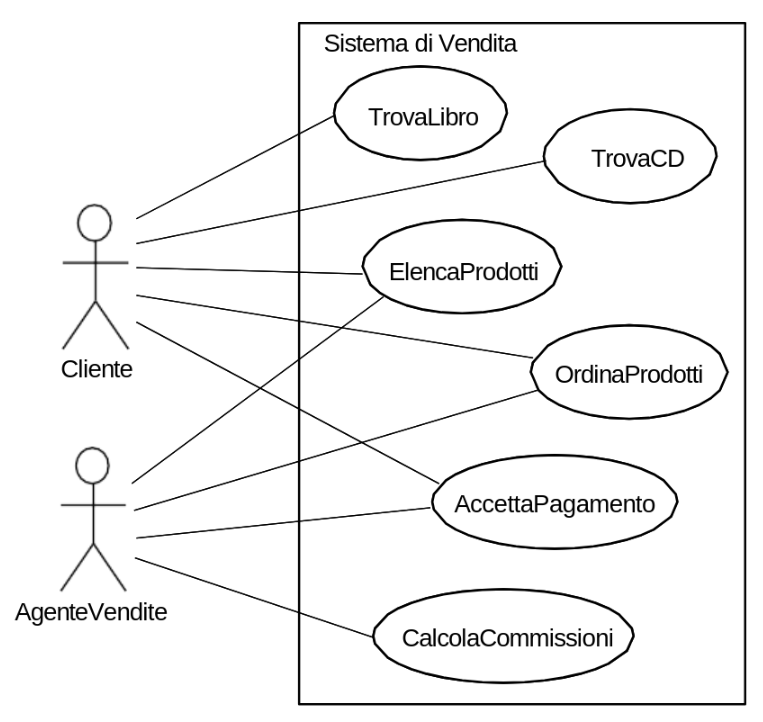
\includegraphics[scale=0.35]{../figures/assoc_attori_casi_uso.png}
\end{center}

	\item La complessità data da più attori che interagiscono con gli stessi casi d'uso può essere ridotta introducendo la \textbf{generalizzazione degli attori}: più \textit{sottoattori} potrebbero ereditare relazioni con casi d'uso da un \textit{superattore} comune e \textit{generico}.
		Riguardo all'esempio precedente, vediamo come si può introdurre un \textit{Acquirente}:
\begin{center}
	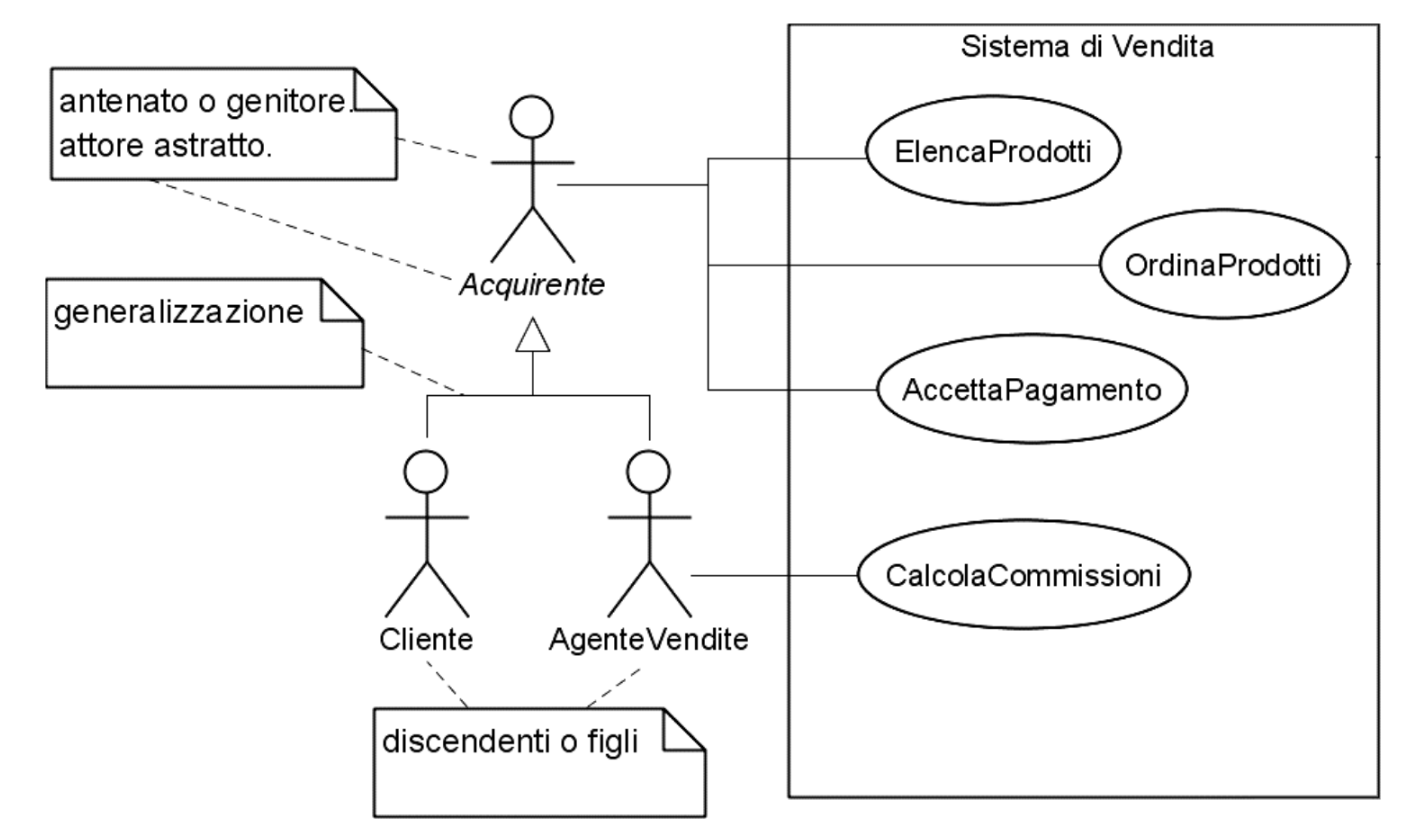
\includegraphics[scale=0.3]{../figures/general_attori_casi_uso.png}
\end{center}
Gli attori \textit{Cliente} e \textit{AgenteVendite} diventano a questo punto generalizzazioni di \textit{Acquirente}.
Notiamo come questo ci permette di spiegare elegantemente come mai entrambi gli attori sono interessati a casi d'uso comuni come \textit{ElencaProdotti}, ecc...

	\item Come si generalizzano gli attori, potrebbe essere utile stabilire la \textbf{generalizzazione dei casi d'uso}: i sottocasi ereditano tutte le caretteristiche (relazioni, punti d'estensione, precondizioni, postcondizioni, flussi principali e alternativi) del supercaso, e possono sovrascriverle (tranne relazioni e punti d'estensione).
		Ad esempio, nell sistema visto finora si potrebbe voler generalizzare il caso d'uso \textit{TrovaProdotto} sulla base del prodotto cercato:
\begin{center}
	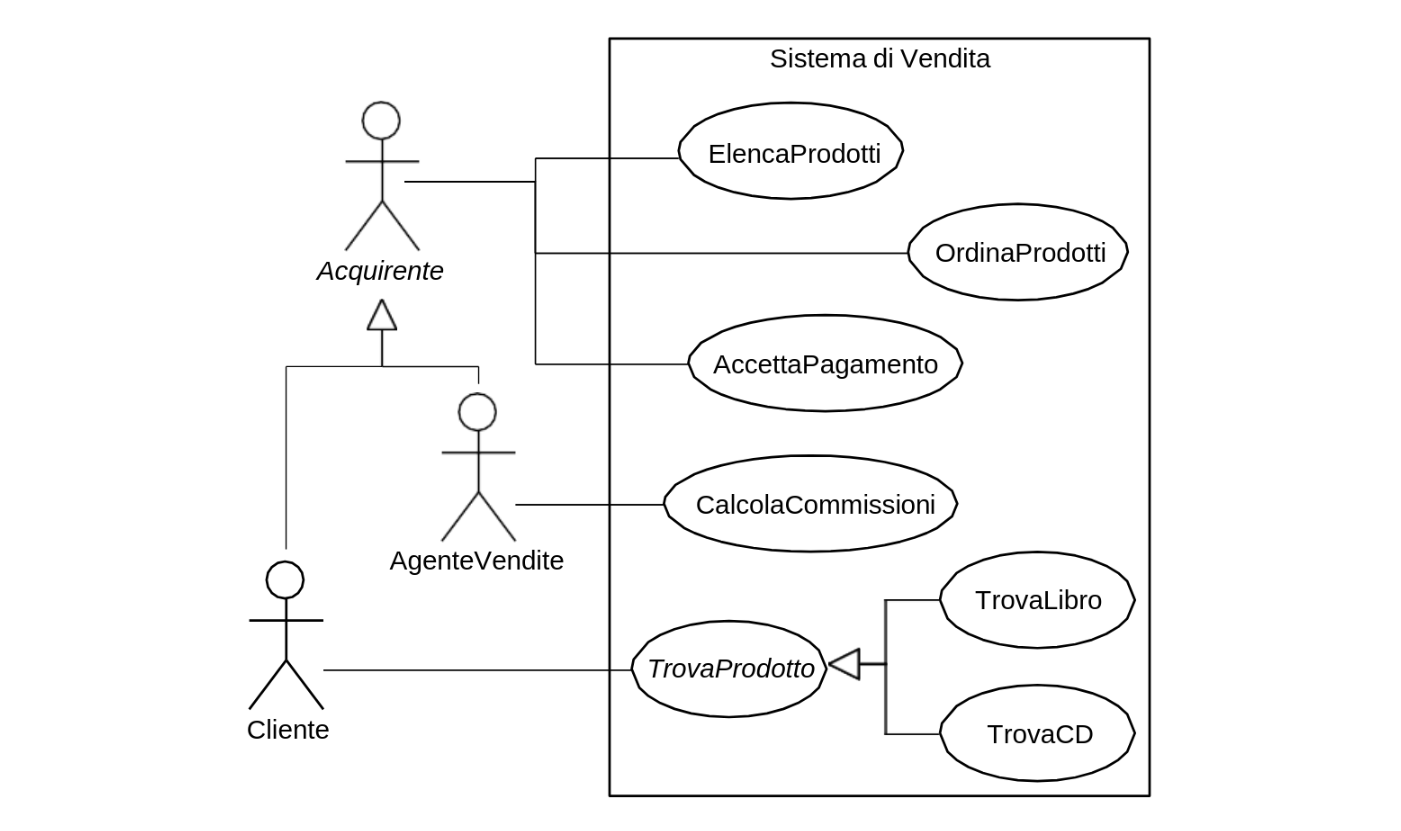
\includegraphics[scale=0.35]{../figures/general_casi_uso.png}
\end{center}

		Potrebbe essere utile definire alcune regole su come i sottocasi possono sovrascrivere i flussi dei supercasi, assunti questi come liste di operazioni:
		\begin{itemize}
			\item Si indicano fra parentesi le operazioni ereditate, ad esempio 3. (3.) o 4. (3.) se si è rinumerata;
			\item Si prefiggono con una "o" loe operazioni sovrascritte, ad esempio 3. (o3.) o 4. (o3.) se si è rinumerata;
			\item Infine, le operazioni aggiunte da zero si indicano semplicemente con numeri non usati nel supercaso. 
		\end{itemize}
	\item Se si prevedono casi d'usi e attori "figli", possiamo anche prevedere casi d'uso e attori \textbf{astratti}, cioè incompleti e pensati per definire caratteristiche base. In particolare, preferiamo definire i \textbf{casi d'uso astratti} come casi d'uso con sequenze di operazioni incomplete e da definire, mentre gli \textbf{attori astratti} possono essere una variante più forte degli \textit{attori generici} visti quando abbiamo introdotto la \textit{generalizzazione degli attori}. 
\end{itemize}

\subsubsection{Relazioni \lstinline|<<include>>| e \lstinline|<<extend>>|}
Altri due meccanismi di estensione della modellizzazione dei casi d'uso sono rappresentati dalle relazioni \lstinline|<<include>>| e \lstinline|<<extend>>|. Abbiamo che queste relazioni sollevano la specifica del flusso dalle relazioni di ereditarietà fra casi d'uso, mantenendo solo il collegamento semantico. Vediamole nel dettaglio:
\begin{itemize}
	\item La relazione \lstinline|<<include>>| definisce, appunto, l'\textit{inclusione} di un caso d'uso (detto \textbf{caso d'inclusione}) all'interno di un altro (detto \textbf{caso base}). Dal punto di vista del programmatore, il caso d'inclusione rappresenta un frammento di comportamento che viene ripetuto in più casi d'uso base allo stesso modo (la corrispondenza più significativa dal lato implementativo è una banale chiamata di funzione).

		Un esempio di inclusione di casi d'uso potrebbe essere il seguente:
\begin{center}
	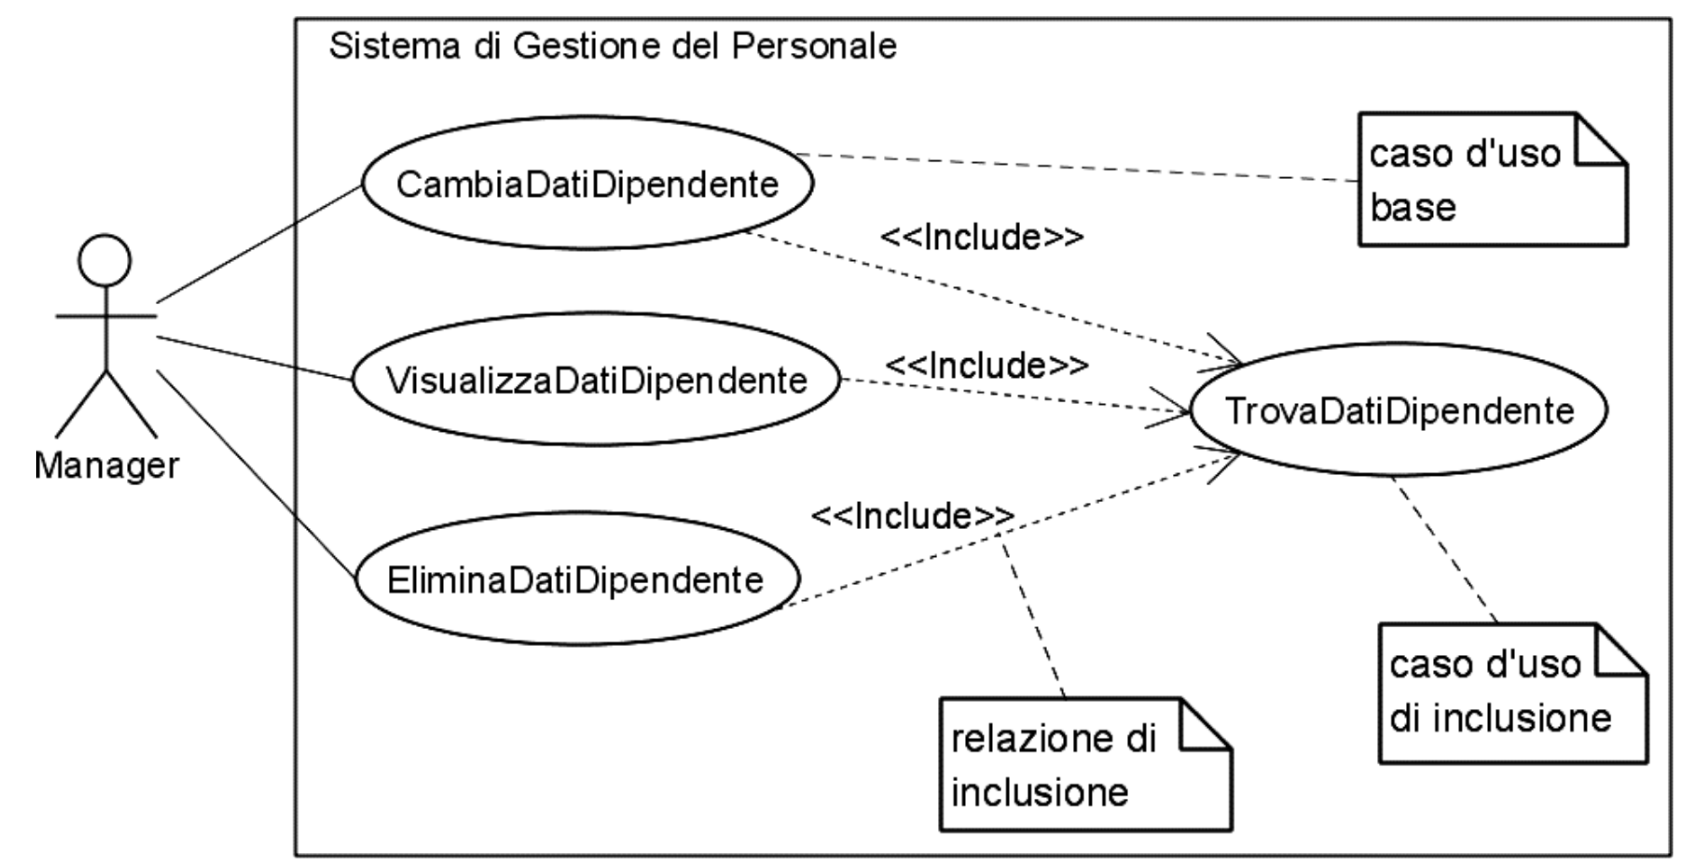
\includegraphics[scale=0.25]{../figures/include_casi_uso.png}
\end{center}
		dove il frammento di comportamento \textit{TrovaDatiDipendente} è incluso nei casi d'uso \textit{CambiaDatiDipendente}, \textit{VisualizzaDatiDipendente}, \textit{EliminaDatiDipendente}.

		Abbiamo che sicuramente i casi base non sono completi senza casi d'inclusione. Di contro, anche i casi di inclusione possono essere incompleti senza un caso base che li includa: in questo caso si dicono \textbf{non istanziabili}.

	\item La relazione \lstinline|<<extend>>| definisce una relazione apparentemente simile all'inclusione, ma più legata alla gestione di eccezioni ai flussi principali: definiamo infatti \textbf{punti di estensione} i punti di un flusso dove si può aggiungere comportamento. In questo, i \textbf{casi di estensione} \textit{estendono} i \textbf{casi base} nei punti di estensione. Nulla nega che lo stesso caso d'estensione estenda più punti d'estensione.

		Per approfondire, abbiamo che ogni caso d'uso d'estensione non è completo, e consiste di più frammenti detti \textbf{segmenti di inserzione}. Ogni segmento di inserzione deve combaciare con un punto d'estensione del caso base che si va ad estendere. Inoltre, si può avere che due casi di estensione estendono lo stesso punto d'estensione: in questo caso si prevedono più comportamenti d'estensione, il cui ordine di esecuzione è indeterminato.

\newpage

		Vediamo come si possono estendere i casi d'uso degli esempi precedenti introducendone uno, \textit{EmettiMulta}, e usandolo per estendere i flussi alternativi di fallimento:
\begin{center}
	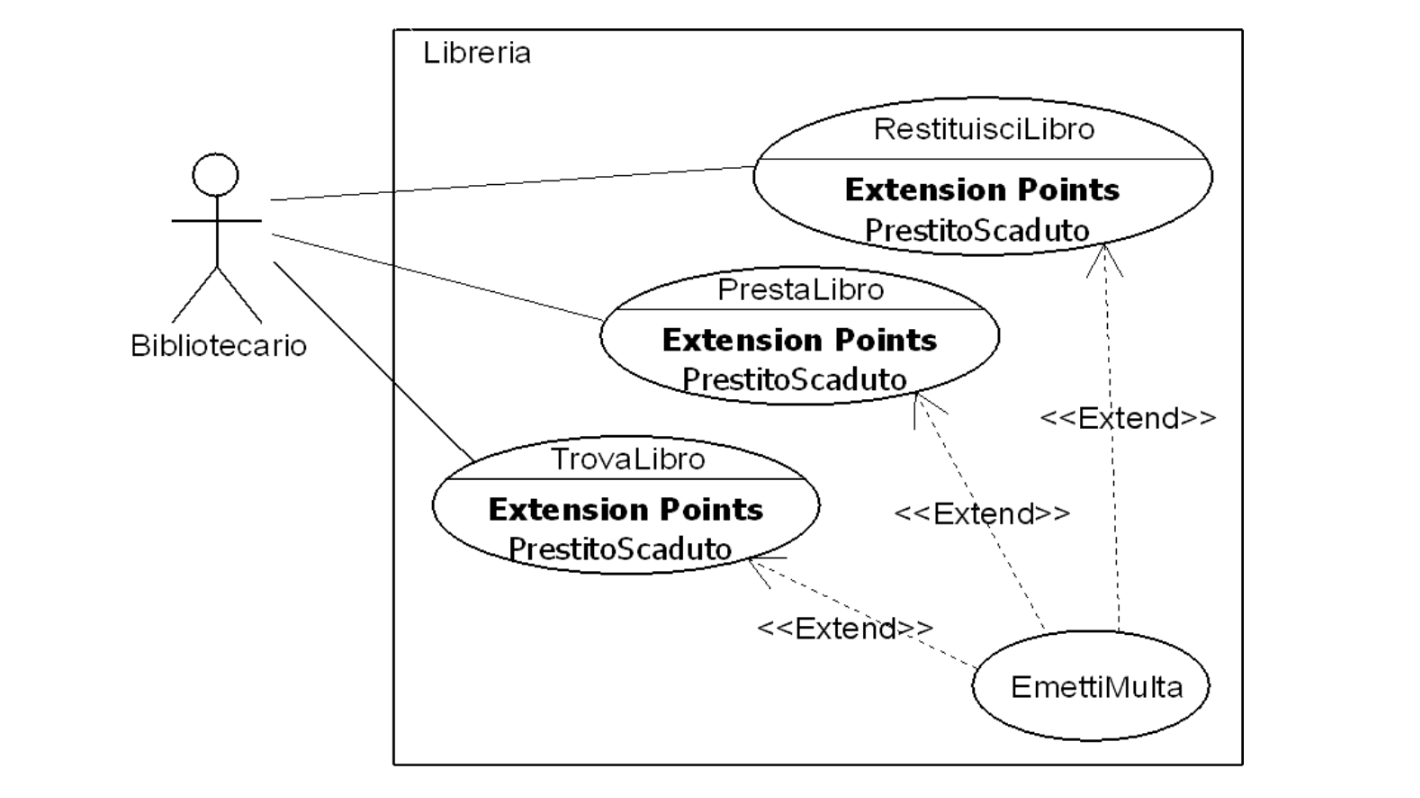
\includegraphics[scale=0.35]{../figures/extend_casi_uso.png}
\end{center}

		Infine, abbiamo che i casi di estensione possonoo essere vincolati da \textit{precondizione}, e vincolare lo stato successivo del sistema dopo la loro esecuzione attraverso \textit{postcondizioni}. Per completare il quadro assieme all'esempio fatto sopra, la corrispondenza implementativa più banale è quella di una chiamata condizionale di funzione.
\end{itemize}

\subsection{Workflow analisi}
Il workflow analisi ha il compito di creare un modello che catturi \textit{cosa} il sistema deve fare (il \textit{come} è prerogativa del workflow progetto).
Gli artefatti prodotto in questo workflow sono:
\begin{itemize}
	\item \textbf{Classi di analisi}: modellano i concetti chiave del soggetto;
	\item \textbf{Realizzazioni di casi d'uso}: illustrano com ele istanze delle classi di analisi possono interagire per realizzare i casi d'uso registrati nel workflow requisiti.
\end{itemize}

In questo caso, questa parte corrisponde con le \textit{strutture statiche} e il \textit{comportamento dinamico} che avevamo discusso in 2.1.

\subsubsection{Classi e oggetti}
Un'\textbf{oggetto} è un entità discreta con un confine ben definito che ne incapsula stato e comportamento.
La struttura dell'oggetto e il modo	in cui ci si interagisce sono definite dalla \textbf{classe} dell'oggetto.
La classe si distingue dall'oggetto in quanto l'oggetto è un \textbf{istanza} della classe.

Tutti gli oggetti hanno \textbf{proprietà} comuni:
\begin{itemize}
	\item \textbf{Identità}: un numero o qualche altro identificativo che individua univocamente l'oggetto. Per quanto ci riguarda, un \textit{riferimento} all'istanza di classe;
	\item \textbf{Stato}: determinato dallo stato interno corrente dell'oggetto e le relazioni che al momento questo ha con altri oggetti. Per quanto ci riguarda, il valore dei \textit{campi} dell'oggetto;
	\item \textbf{Comportamento}: le operazioni che l'oggetto può compiere. Chiaramente, questo può essere influenzato dallo stato corrente dell'oggetto. Per quanto ci riguarda, sono i \textit{metodi} dell'oggetto.
\end{itemize}

Vediamo quindi come l'UML mira a modellizzare sistemi \textbf{orientati agli oggetti}, dove più oggetti \textit{istanze} di \textit{classi} interagiscono (\textbf{scambiano messaggi}) mantenendo privato il loro stato interno (\textbf{incapsulamento}).

\subsubsection{Notazione di oggetti}
In UML per identificare oggetti si usa un formato tabulare del tipo:
\begin{table}[H]
	\center 
	\begin{tabular} { | c | }
		\hline
		\underline{nomeIstanza : Classe} \\
		\hline
		attributo : tipo = letterale \\
		... \\
		\hline
	\end{tabular}
\end{table}
dove notiamo che:
\begin{itemize}
	\item L'identificatore di oggetto è sempre sottolineato;
	\item Il nome dell'oggetto può essere risparmiato nel caso di \textit{oggetti anonimi};
	\item L'identificatore può di contro essere composto solo dal nome dell'oggetto: questo è utile in fase di analisi prima che una classe vera e propria venga definita.
\end{itemize}

Le operazioni defnite sull'oggetto non vengono riportate in quanto sono comuni a tutte le istanze di classe (vanno cercate nella definizione di classe). 

\subsubsection{Notazione di classi}
Per identificare classi in UML si usa ancora una volta una struttura tabulare:
\begin{table}[H]
	\center 
	\begin{tabular} { | c | }
		\hline
		<<entità>> \\ 
		Classe \\
		\hline
		\textit{Comparto attributi}: \\ 
		- attributo : tipo \\
		... \\ 
		\hline
		\textit{Comparto operazioni}: \\ 
		- operazione(argomento : tipo, ...) \\ 
		... \\
		\hline
	\end{tabular}
\end{table}
dove notiamo che:
\begin{itemize}
	\item Distinguiamo in \textit{comparto attributi} e \textit{comparto operazioni}:
		\begin{itemize}
			\item \textit{Comparti attributi}: la visibilità viene solitamente omessa. A volte, si possono usare gli ornamenti (+, -, $\#$, $\sim$), che corrispondono a (\textit{public}, \textit{private}, \textit{protected}, \textit{package} (o \textit{friendly})). Inoltre, si può indicare una \textit{molteplicità}, che per i nostri scopi definisce array;
			\item \textit{Comparti operazioni}: di queste si possono definire i parametri in entrata e in uscita usando le parole chiave \lstinline|in|, \lstinline|out| e \lstinline|inout| nella lista degli argomenti.
		\end{itemize}
\end{itemize}

Notiamo inoltre che si possono definire operazioni specifiche all'implementazione del paradigma OOP (tipicamente il \textbf{costruttore}), e che si possono sottolineare i membri, in qualsiasi comparto, che hanno \textbf{visibilità di classe}.
Quest'ultima caratteristica è per noi assimilabile all'idea dei membri \textit{statici}: come sappiamo la classe può accedere ai suoi membri statici, mentre le istanze possono accedere sia ai membri di istanza che ai membri statici.

\par\smallskip

Una volta definite classi e istanze di queste, si può usare la relazione \lstinline|<<instantiate>>| (diretta da istanza a classe) per definirne la dipendenza.

\subsubsection{Trovare le classi}
Il problema fondamentale del design OOP diventa quindi trovare tassonomie di classi che descrivono bene il soggetto e implementano con relazioni semplici e compatte i casi d'uso.
Non esiste una metodologia prefissata per lo sviluppo di tali tassonomie. Alcuni metodi che possiamo usare sono:
\begin{itemize}
	\item Analisi \textbf{nomi-verbi}: i nomi ed i verbi nel testo indicano rispettivamente classi e responsabilità. Chiaramente, questo metodo richiede una buona conoscenza del soggetto, un buon glossario (in modo da individuare sinonimi ed omonimi), e potrebbe richiedere ulteriori fasi di elaborazioni delle classi candidate trovate (magari fusioni di classi simili, rimozione di classi inutili, ecc...);
	\item Analisi \textbf{CRC} (\textit{Classe, Responsabilità, Collaboratore}): possiamo intendere questo metodo come estensione del precedente. Per \textit{collaboratori} si intendono altre classi che possono collaborare con la classe definita per realizzare parte della funzionalità del sistema;
	\item Analisi \textbf{RUP} (\textit{Rational Unified Process}): questa tecnica si basa sull'individuare classi sulla base di tre modelli:
		\begin{itemize}
			\item Classi \textbf{boundary} (\textit{confine}): mediano l'interazione tra soggetto e attori esterne. Rappresentano quindi interfacce, che siano con gli utenti, con altri sistemi o con dispositivi fisici;
			\item Classi \textbf{control} (\textit{controllo}): rappresentano controllori che mediano il comportamento associato a casi d'uso. Queste non devono essere troppo grandi, ed anzi è buona pratica suddividerle in più unit funzionali;
			\item Classi \textbf{entity} (\textit{entità}): caso principe dell'OOP, queste modellano oggetti reali all'interno del soggetto. Vengono gestite dalle classi di controllo per implementare i casi d'uso, e vengono scambiate fra le classi di confine.
		\end{itemize}
\end{itemize}

Oltre a queste metodologie si possono individuare le classi sfruttando oggetti fisici, documenti d'ufficio, usando interfacce, adottando modellizzazioni in \textit{componenti} del soggetto o entità concettuali.

\subsubsection{Relazioni fra classi}
Una volta individuate le classi, cioè la struttura \textit{statica} del sistema, è opportuno definire la natura \textit{dinamica} della collaborazione che ci aspettiamo fra le stesse.
Questa si definisce attraverso \textbf{collegamenti} fra \textit{oggetti} e \textbf{associazioni} fra \textit{classi}.

Per definire i collegamenti bisogna usare un linguaggio sollevato delle specifiche del linguaggio di programmazione, come i \textbf{diagrammi ad oggetti} dell'UML:
\begin{center}
	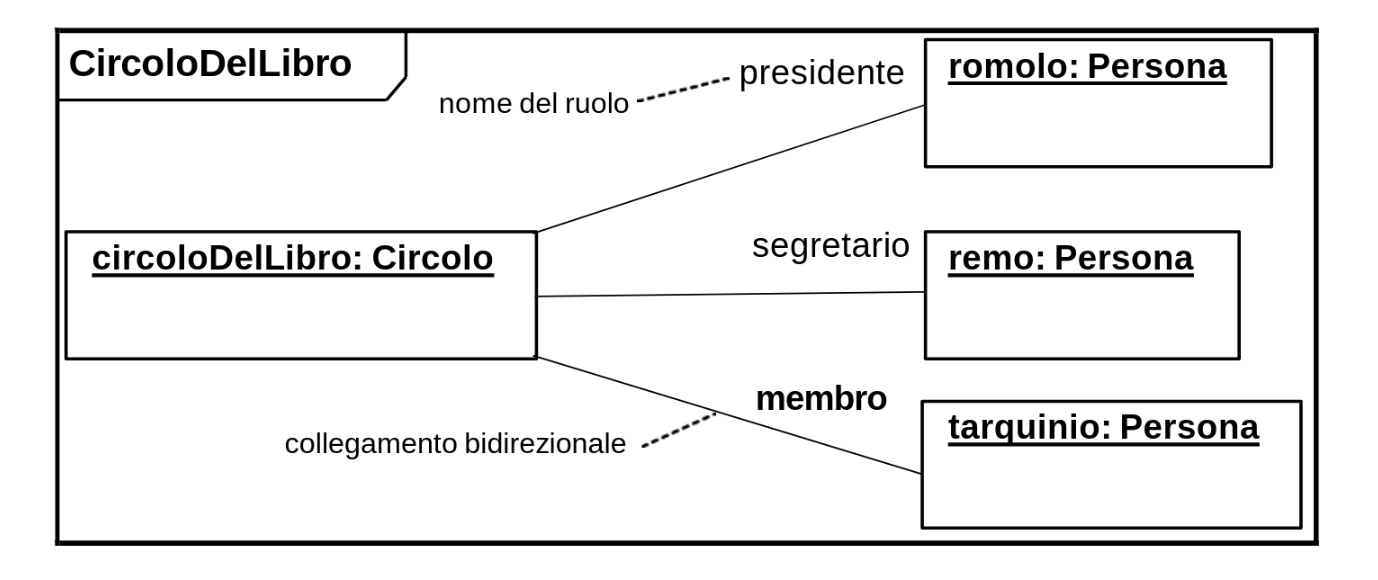
\includegraphics[scale=0.3]{../figures/diag_oggetti.png}
\end{center}

I \textit{collegamenti} in UML sono \textbf{dinamici} (non fissi nel tempo), possono essere \textbf{bidirezionali} o \textbf{monodirezionali}, e devono essere supportati da una \textit{associazione} fra classi.

Le \textit{associazioni} sono solitamente più sofisticate nei diagrammi, e collegate ai rispettivi collegamenti da relazioni \lstinline|<<instatiate>>|. Nelle associazioni vogliamo definire una stringa che definisce l'associazione, i \textbf{ruoli} delle classi coinvolte, e magari indicazioni sulla \textbf{molteplicità} dell'associazione (uno a uno, uno a molti, molti a molti e via dicendo).

Vediamo quindi come \textit{associzioni} e \textit{collegamenti} sono schematizzabili rispettivamente fra \textbf{classi} e \textbf{oggetti}, cioè:
\begin{center}
	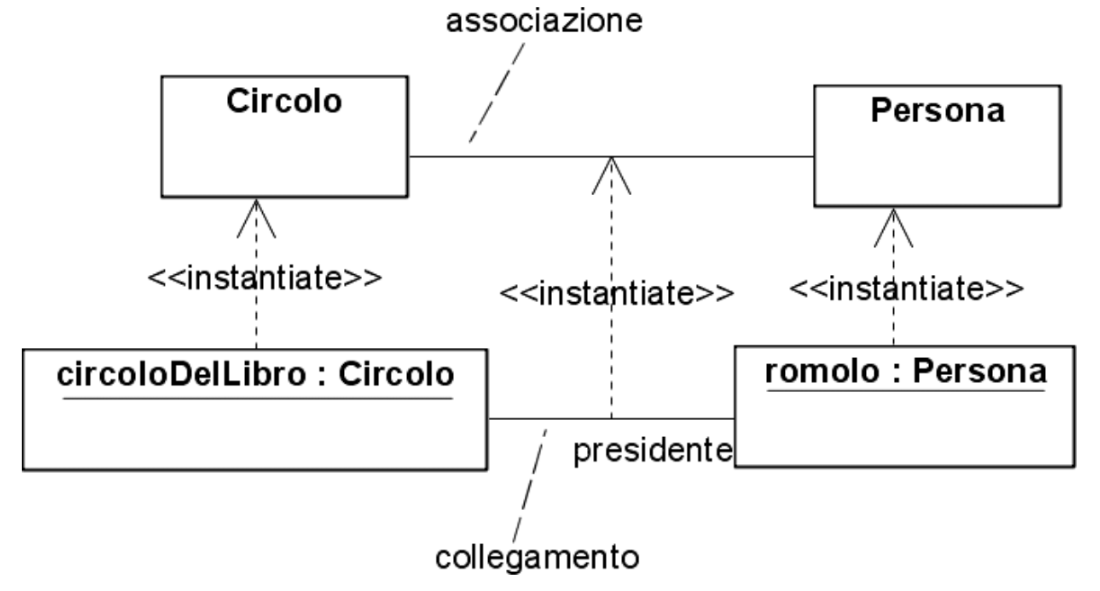
\includegraphics[scale=0.3]{../figures/assoc_colleg.png}
\end{center}

La molteplicità può poi essere supportata dalla \textbf{navigabilità} dell'associazione, intesa nei nostri scopi come la possibilità di raggiungere una classe a partire da quella a cui è associata.
Dovrebbe apparire chiaro come, ad esempio, una classe che contiene un riferimento ad un'altra ci permette di navigare verso questa, e non viceversa.
Il sistema di navigabilità di UML 2.0 è comunque più sofisticato di quanto effettivamente necessario, e le associazioni \textit{bidirezionali} e \textit{monodirezionali} bastano spesso a riassumere tutta la funzionalità di cui abbiamo bisogno.

\subsubsection{Associazioni ed attributi}
L'assocazione fra classi può essere espressa anche come particolari attributi di classe (relazioni uno a uno sono riferimenti, uno a molto array di riferimenti, ecc...).
In questo caso conviene adottare la regola: se la classe associata è parte integrante del modello, usare un'associazione, altrimenti un'attributo.

\subsubsection{Classi di associazioni}
Se l'associazione è molti a molti potrebbero sussistere dei campi che si perdono nella semplice specifica di associazione.
In questo caso può essere utile costruire \textbf{classi di associazione}, che contengono riferimenti ad ognuna delle classi impegnate nell'associazione, e i campi associati a questa.

\subsubsection{Associazioni qualificate}
Le associazioni uno a molti possono essere qualificate da un particolare \textbf{qualificatore}, cioè un particolare indice che ci permette di trasformare la relazione in uno a uno, navigando verso la classe associata.
L'esempio tipico è il qualificatore \textit{codice fiscale} per una classe che si associa a più classi individuo.  

\subsubsection{Dipendenza}
Una dipendenza è una particolare relazione tra due elementi, dove la modifica di un elemento (detto \textbf{fornitore}) può influenzare l'altro elemento (detto \textbf{cliente}).
Esistono 3 tipi di dipendenze in UML:
\begin{itemize}
	\item Dipendenza di \textbf{uso}: se il cliente usa alcuni servizi messi a disposizione dal fornitore. Questa si divide a sua volta in:
		\begin{itemize}
			\item \lstinline|<<use>>|: il cliente usa in qualche modo il fornitore;
			\item \lstinline|<<call>>|: il cliente invoca un'operazione eseguita dal fornitore;
			\item \lstinline|<<parameter>>|: il fornitore è parametro di un'operazione del cliente;
			\item \lstinline|<<send>>|: il cliente invia il fornitore a qualche altro bersaglio;
			\item \lstinline|<<instantiate>>|: il cliente è un'istanza del fornitore, già vista.
		\end{itemize}	
	\item Dipendenza di \textbf{astrazione}: se le entità sono a livelli di astrazione diversi. Questa si divide a sua volta in:
		\begin{itemize}
			\item \lstinline|<<trace>>|: cliente e fornitore rappresentano lo stesso oggetto ma in modelli diversi;
			\item \lstinline|<<substitute>>|: il cliente può sostituire il fornitore;
			\item \lstinline|<<refine>>|: simile a \lstinline|<<trace>>|, ma riferito ad un'ottimizzazione all'interno dello stesso modello;
			\item \lstinline|<<derive>>|: il cliente può essere derivato in qualche modo dal fornitore.
		\end{itemize}
	\item Dipendenza di \textbf{permesso}: modella la capacità di un’entità di accedere ad un’altra entità. Questa si divide a sua volta in:
		\begin{itemize}
			\item \lstinline|<<access>>|: il cliente può accedere ai contenuti pubblici del fornitore, si riferisce principalmente ai \textit{package};
			\item \lstinline|<<import>>|: simile al precedente ma con la fusione dello spazio dei nomi;
			\item \lstinline|<<permit>>|: permette la violazione dell'incapsulamento in linguaggi come il C++ (pensa funzioni e classi \lstinline|friend|).
		\end{itemize}
\end{itemize}

\subsubsection{Ereditarietà}
La \textbf{generalizzazione} o \textit{ereditarietà} è la forma più forte di dipendenza.
Questa indica che un entità cliente (detta \textit{specializzata}) può essere usata in qualsiasi contesto dell'entità fornitore (detta \textit{base}), con la differenza che l'entità cliente definisce informazioni e procedure aggiuntive rispetto all'entità fornitore.

Facciamo l'esempio classico di un \textbf{diagramma di ereditarietà} che definisce una \textit{tassonomia} di classi (cioè) il modo in cui più classi ereditano funzionailtà l'una dall'altra, dall'alto verso il basso:
\begin{center}
	\begin{forest}
		[Animal, rectstyle
			[Dog
				[Bulldog]
				[Chihuaha]
				[Hound]
			]
			[Bear]
			[Axolotl]
		]	
	\end{forest}
\end{center}

In particolare, in questo caso vogliamo usare l'ereditarietà per modellare una relazione \lstinline|<<is-a>>| (\textit{"è un"}): un bulldog \textit{è un} cane, che a sua volta \textit{è un} animale, e cosi via.

Sfruttando l'ereditarietà riusciamo quindi a modellare bene il tipo di categorizzazioni che incontreremo naturalmente nel soggetto del sistema che andiamo a sviulppare.

\subsubsection{Polimorfismo}
L'idea del \textbf{polimorfismo} è simile a quella dell'ereditarietà, e indica contesti dove si può inviare lo stesso messaggio a entità di classe differente e aspettarsi risposte semanticamente appropiate.

Per fissare i concetti, una classe base \textit{Veicolo} può essere \textbf{generalizzata} in \textit{Camion}, \textit{Elicottero}, ecc... la possibilità di inviare a tutte queste il segnale \textit{guida()} è un'esempio di \textbf{polimorfismo}:
\begin{center}
	\begin{forest}
		[Conducente, rectstyle
			[Camion, edge label={node[midway,left]{guida()}}]
			[Elicottero, edge label={node[midway,right]{guida()}}]
		]	
	\end{forest}
\end{center}

Chiaramente, in un linguaggio di programmazione reale si dovranno usare i costrutti tipici dell'OOP per realizzare la stessa funzionalità, come classi o membri \textit{astratti} e il meccanismo dell'\textit{overriding}.

\end{document}
